%	01.01.01. Formas de presentaci\'on informaci\'on
%	version 2018



\begin{frame}{Formas de presentaci\'on de la informaci\'on}

  \begin{itemize}
  \item {\bf Presentaciones cuantitativas}
    \begin{itemize}
      \item Escala circular
      % \begin{itemize}
      %    \item Escala lineal
      %    \item Escala no lineal (cuadr\'atica, logar\'itmica}
      % \end{itemize}
       \item Escala longitudinal
    \end{itemize}
  \item {\bf Presentaciones cualitativas}
  \item {\bf Presentaciones directoras}
  \end{itemize}

\end{frame}

\begin{frame}{Presentaciones cuantitativas
	}

  \begin{tabular}{ccc}
    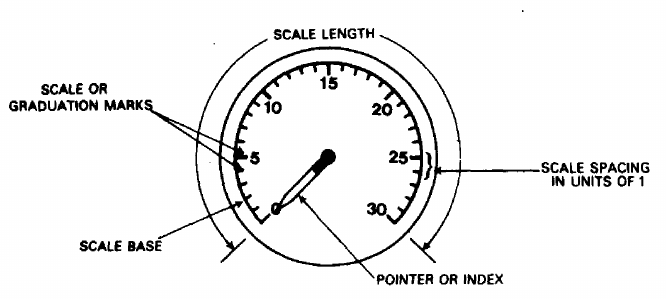
\includegraphics[width=0.45\textwidth]{imagenes/1.2.clasificacion.instrumentos/escala_circular_cuantitativa.png} & \hspace{3mm}
&     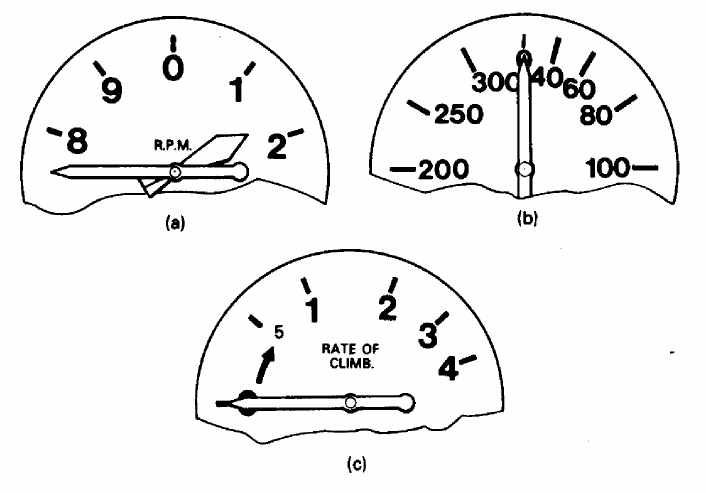
\includegraphics[width=0.45\textwidth]{imagenes/1.2.clasificacion.instrumentos/escala_circular_lineal_no_lineal.png}
\\
	Escala circular cuantitativa & 
& \parbox{0.45\textwidth}{a) Lineal, b) ley cuadr\'atica, \\c) ley logaritmica}
\\
  \end{tabular}

{\tiny Referencia: \cite{pallett1992aircraft}}

\end{frame}

\begin{frame}{Presentaciones cuantitativas
	}

  \begin{tabular}{ccc}
    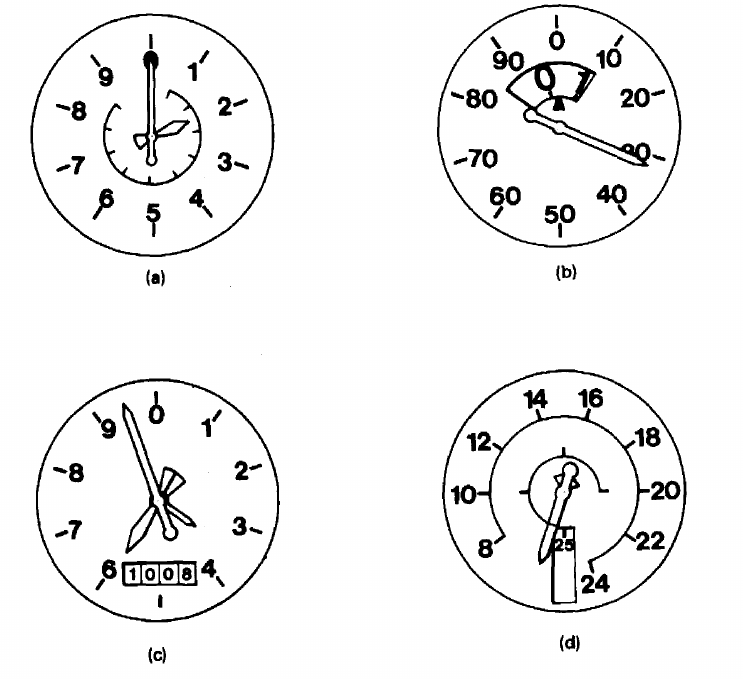
\includegraphics[width=0.45\textwidth]{imagenes/1.2.clasificacion.instrumentos/escala_gran_alcance.png} & \hspace{3mm}
&     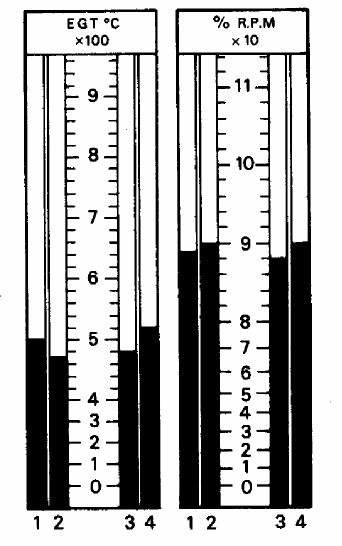
\includegraphics[width=0.35\textwidth]{imagenes/1.2.clasificacion.instrumentos/longitudinal.png}
\\
\parbox{0.45\textwidth}{\small a)Escalas conc\'entricas, (b) escalas fijas y giratorias, (c) escala com\'un tres agujas, (d) aguja dividida}
&
& {\small Escala longitudinal}
\\
  \end{tabular}
{\tiny Referencia: \cite{pallett1992aircraft}}
\end{frame}

\begin{frame}{Clasificaci\'on de los Instrumentos}

  \begin{tabular}{ccc}
    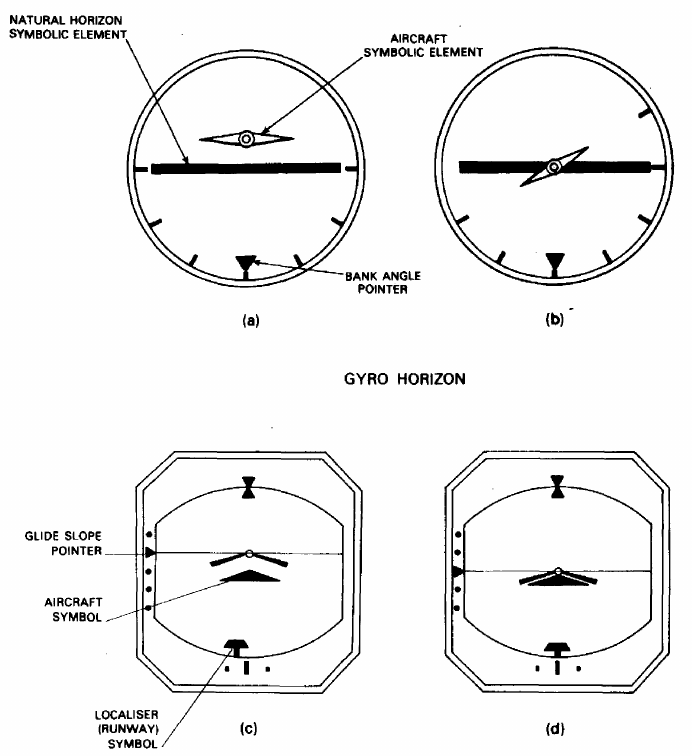
\includegraphics[width=0.45\textwidth]{imagenes/1.2.clasificacion.instrumentos/director.png} & \hspace{3mm}
&     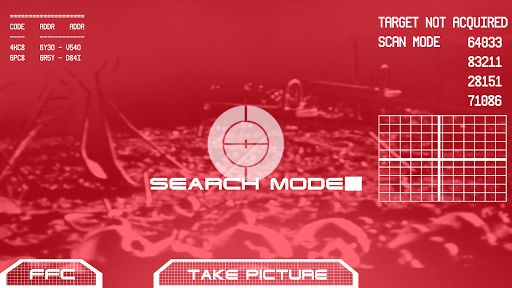
\includegraphics[width=0.5\textwidth]{imagenes/1.2.clasificacion.instrumentos/terminator_hud.png}
\\
\parbox{0.45\textwidth}{Director de vuelo}
&
& Terminator Hud
\\
  \end{tabular}

\end{frame}

\begin{frame}{Clasificaci\'on de los Instrumentos}

{
\includegraphics[width=0.1\textwidth]{imagenes/Video.png}}\,
The Evolution of the Head-Up Display \url{https://www.youtube.com/watch?v=ypIbmfm7n8A}
\vspace{3mm}

  \begin{tabular}{ccc}
    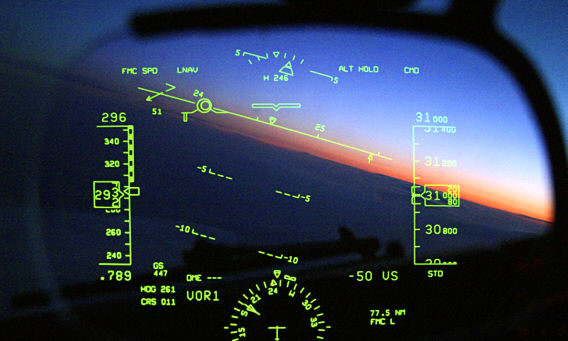
\includegraphics[width=0.45\textwidth]{imagenes/1.2.clasificacion.instrumentos/hud.jpg} & \hspace{3mm}
&     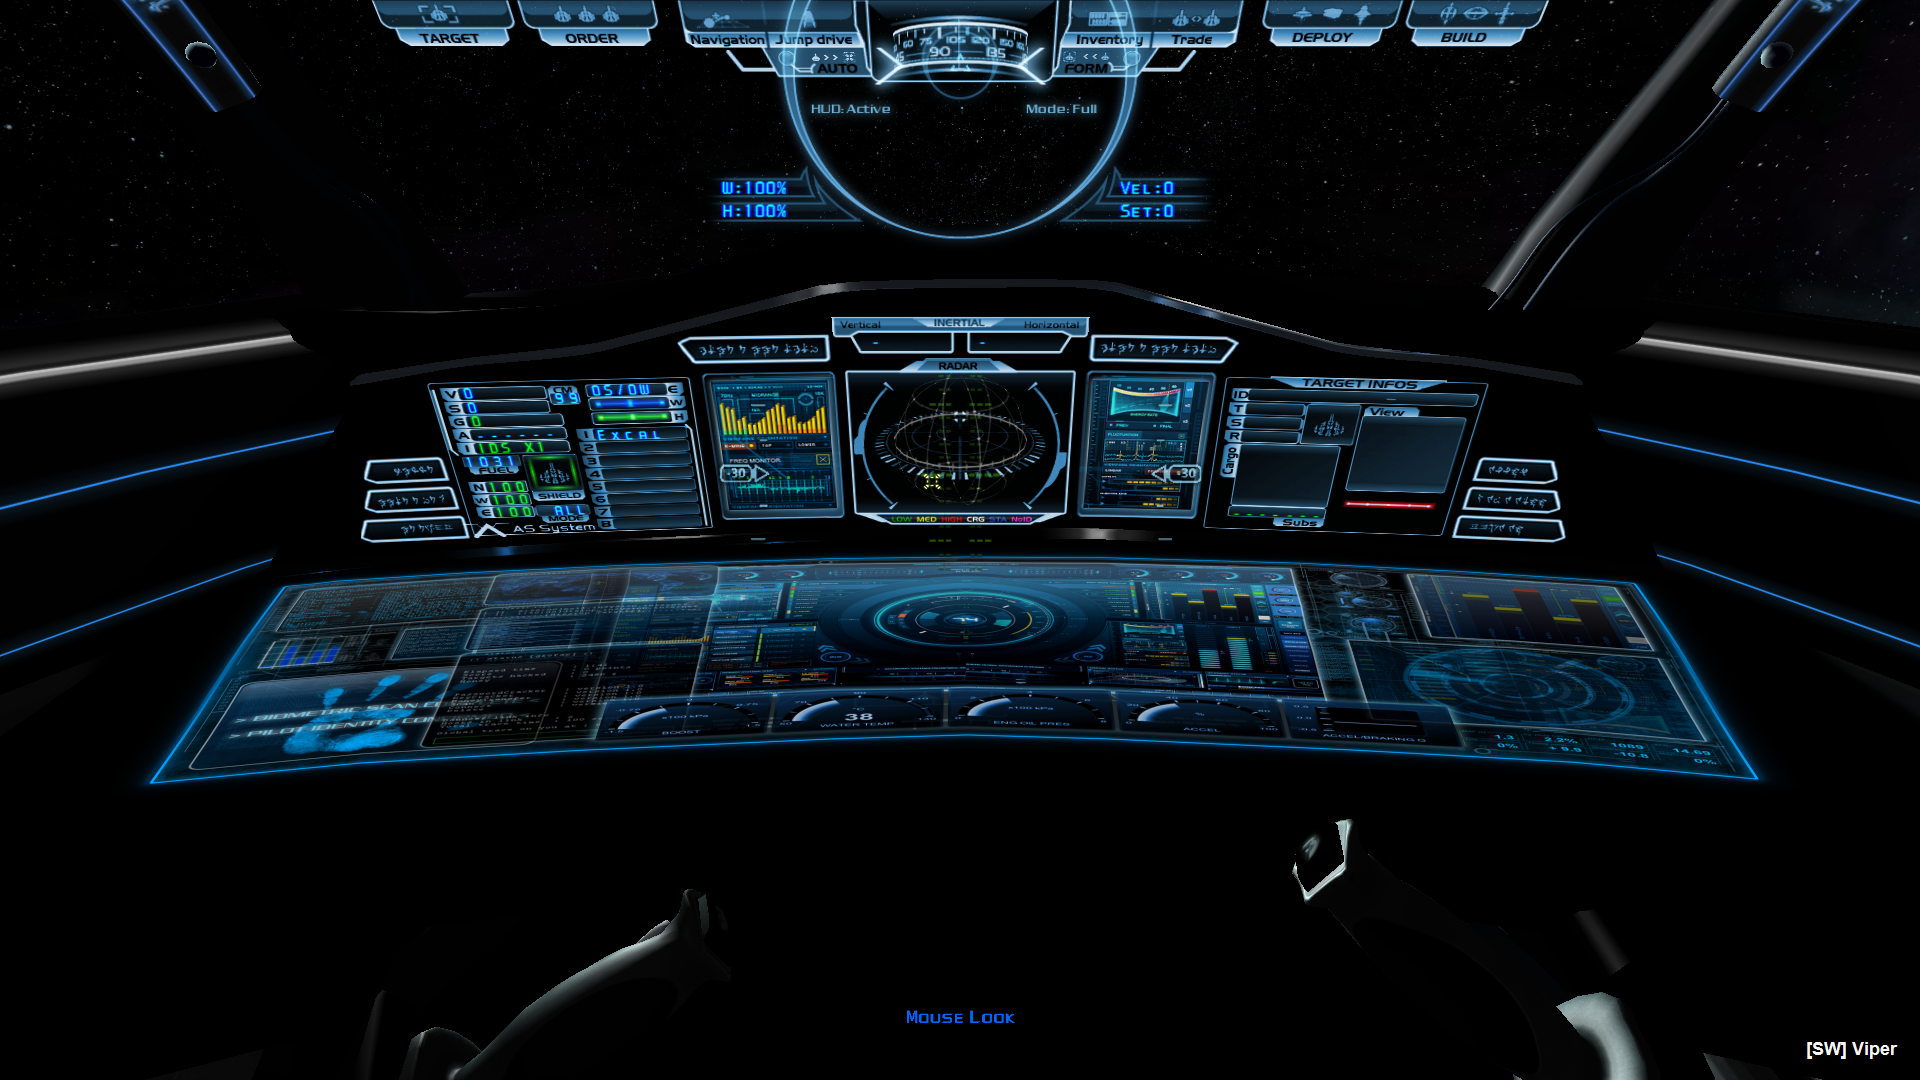
\includegraphics[width=0.5\textwidth]{imagenes/1.2.clasificacion.instrumentos/viper_11.png}
\\
\parbox{0.45\textwidth}{Head Up Display}
&
& Hud futuro
\\
  \end{tabular}

\end{frame}

\begin{frame}{Clasificaci\'on de los Instrumentos}



\vspace{3mm}

{
\includegraphics[width=0.1\textwidth]{imagenes/Video.png}}\,
Enhanced Flight Vision System \url{https://www.youtube.com/watch?v=DR9lyAM2YNE}

\vspace{3mm}

  \begin{tabular}{ccc}
    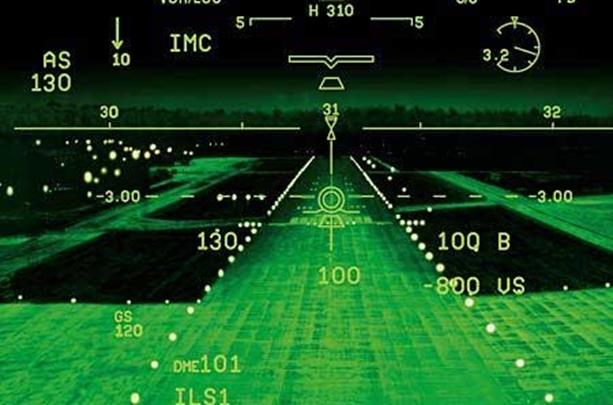
\includegraphics[width=0.45\textwidth]{imagenes/1.2.clasificacion.instrumentos/EFVS_Photo.jpg} & \hspace{3mm}
    &     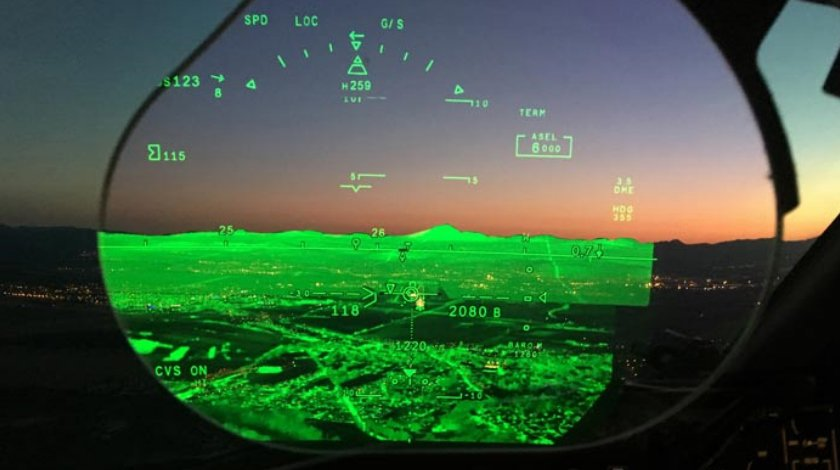
\includegraphics[width=0.45\textwidth]{imagenes/1.2.clasificacion.instrumentos/efvs.jpg} \\
  \end{tabular}
  

\end{frame}
